\documentclass[DIV=15]{scrartcl}


\usepackage{graphicx}
\usepackage{epstopdf} 
\usepackage{amsfonts,amsmath,enumerate,amssymb,bm,siunitx}
\usepackage[numbers]{natbib}



\begin{document}

\section*{Within-Host Stuff}

The within-host dynamics are governed by these equations:
\begin{gather*}
\frac{\text{d} \bm{x}}{ \text{d} t} = (1-k)Q \bm{x} + ar_L \bm{y}-\bm{x} \big((1-k)\bar{\gamma} + a r_L \big), \\
\frac{\text{d} \bm{y}}{ \text{d} t} = \frac{k}{r_L}Q \bm{x} - a \bm{y}-\bm{y} \bigg(\frac{k}{r_L}\bar{\gamma} - a \bigg),
\end{gather*}
where$Q=( q_{ij}) = (m_{ij}\gamma_{ij})$ is the replication-mutation matrix.  $r_L$ is the relative reservoir size, 
$k$ is the rate of entering the reservoir and $a$ the  rate of leaving it. (Also what is $\gamma$?). $\bm{x}$ and $\bm{y}$ are the frequencies of each strain in the active compartment and the reservoir respectively.

\subsection*{PrEP: No Reservoir}
First two strains only are considered: resistant and wild-type.  The fitnesses of the two  strains (replication rates)  are then given by \begin{equation}
(t) = \begin{pmatrix}
1.05(1- C(t)) \\1
\end{pmatrix} , 
\label{gamma}
\end{equation}
where $C(t)$ is relative concentration of the drug (i.e $C=1$ means it is completely effective and $C=0$ has no effect). For now the drug profile is taken to  be as in Figure \ref{drug}. So the person goes onto PrEP shortly after having contracted HIV (at $t=0$) after $6$ months (REF) they are taken of it. It is assumed that at $t=2$ they receive proper treatment (ART).
\begin{figure}[h]
\begin{center}
    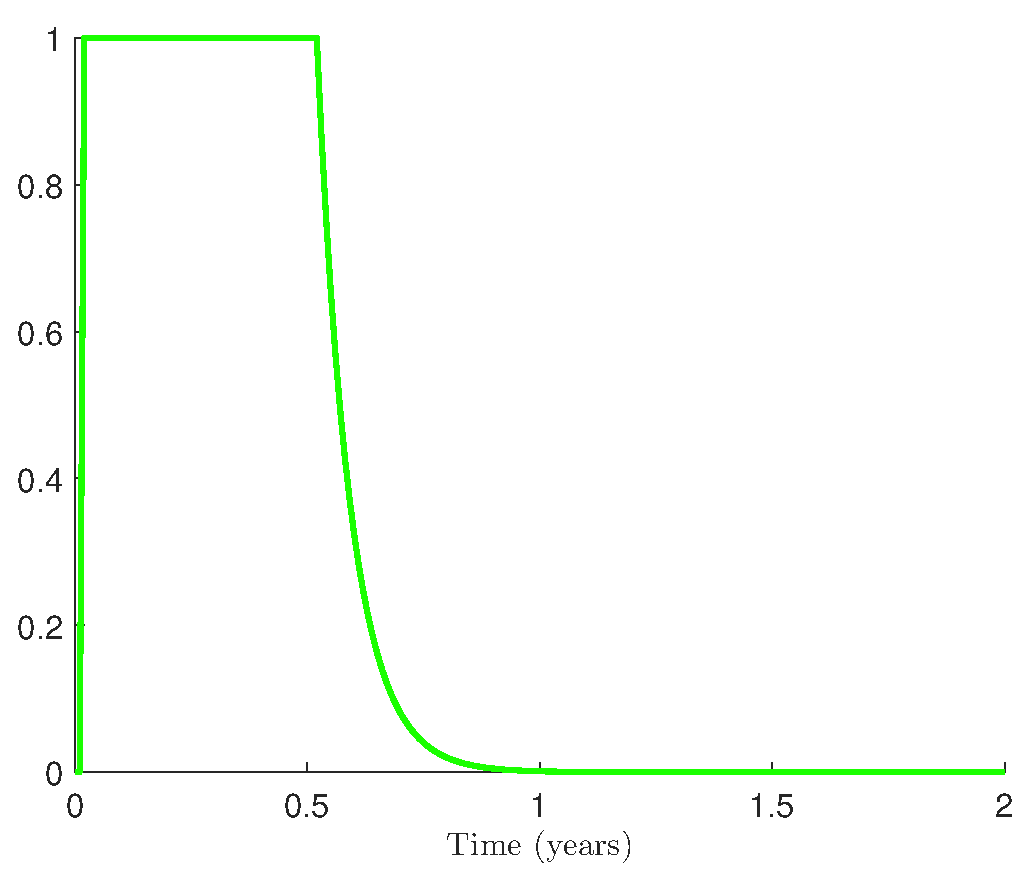
\includegraphics[width=0.5\textwidth]{DrugConc_19_04a.eps}
\end{center}
	\caption{The concentration of drug}
\label{drug} 
\end{figure}
\iffalse
The drug concentration $C$ is given by this, so the virus os contracted shortly (about 1 week) before going onto PrEP. 
After two years we assume  the person goes  onto ART and so is removed from the  susceptible population.
\begin{figure*}
\begin{minipage}{.5\textwidth}
  \includegraphics[width=.4\linewidth]{WithinHost_20_04a.eps}
\end{minipage}%
\begin{minipage}{.5\textwidth}
  \includegraphics[width=.4\linewidth]{WithinHost_20_04b.eps}
\end{minipage}
\caption{}
\label{fig:80}
\end{figure*}
\fi
 Without the reservoir the frequency of the resistant strain  is $0.001$  at $t=2$. At equilibrium we will have A frequency of about $0.0002$, due to the mutations I suppose (this needs to be checked properly),  it's still at $0.001$ at $t=10$. figure \ref{freqwithoutres} shows how the  fitness is affected by the drug.
\begin{figure*}[h]
 \begin{center}$
 \begin{array}{cc}
 \includegraphics[width=.5\linewidth]{WithinHost_20_04a.eps} &
 \includegraphics[width=.5\linewidth]{WithinHost_20_04b.eps}
 \end{array}$
 \end{center}
 \caption{The within-host dynamics in the  absence of the reservoir. The mutation probability is $\SI{5e-5}{}$ per replication and $ \gamma $ is as in equation (\ref{gamma}).}
 \label{freqwithoutres}
 \end{figure*}
 One would hope that the frequency is low enough at $t=2$ that any extra mutations are unlikely to happen.
 
 \subsection*{PrEP: Reservoir}

For a large range of parameter values the presence of the reservoir increases the amount of resistant strain in the active compartment. It is assumed that the founder strain is the wild-type so this may be preferentially passed on REF,so this may need to be accounted for. Also find what is considered to be the most appropriate amount of time to wait until going onto ART and how quickly PrEP is removed from body after treatment ends.
\begin{figure*}[h]
 \begin{center}$
 \begin{array}{cc}
 \includegraphics[width=.5\linewidth]{FrequencyofResistantStraininActiveCompartment_20_04a.jpg} &
 \includegraphics[width=.5\linewidth]{FrequencyofResistantStraininActiveCompartment_20_04b.jpg}
 \end{array}$
 \end{center}
 \caption{Increase in frequency of  the resistant strain present in the active compartment due to the presence of the reservoir. In the left image the homoeostatic proliferation rate is zero ($k = r_L a$). In the right we have $a = 0.01$. With the drug concentration and reproduction rate as before.}
 \label{freqwithres}
 \end{figure*}


\begin{figure*}[h]
 \begin{center}$
 \begin{array}{cc}
 \includegraphics[width=.5\linewidth]{WithinHostActive_20_04a.eps} &
 \includegraphics[width=.5\linewidth]{WithinHostReservoir_20_04a.eps}
 \end{array}$
 \end{center}
 \caption{Strain frequencies in the active compartment and the reservoir for $k = 0.0051$, $a = 0.01$ and $r_L = 2$. The other parameters are the same as before}
 \label{freqwithres}
 \end{figure*}
 
\section*{Between  Host}
To model  the between host effects more than one host type needs to  be considered. Now there are $n$ strains and $m$ host types (use better notation), so the equations are: 
\begin{gather}
H^{(j)}_{i}(t) = \frac{S^{(j)}(t)}{N(t)}  \sum_{k=1}^n \sum_{l=1}^m  \int_0^{T^{(l)}_{k}} \alpha^{(j)}_{k}(\tau) x^{(l)}_{ik}(\tau) H^{(l)}_{k}(t-\tau)e^{-\mu \tau} \ \text{d}\tau \label{multi1} \\
I_i^{(j)}(t) = \int_0^{T_i^{(j)}}  H_i^{(j)}(t-\tau)e^{-\mu \tau} \  \text{d}\tau \\
S(t) = N(t) -  \sum_{k=1}^n \sum_{l=1}^m  I^{(l)}_k(t) \\
\frac{\text{d}}{\text{d} t}  N(t) = B- \mu N(t) -\sum_{k=1}^n \sum_{l=1}^m  H_k^{(l)}(t-T_k^{(l)})e^{-\mu T_k^{(l)}}
\end{gather}
$H^{(j)}_{i}(t)$ is the rate infections initiated with strain $i$ occur in host type $j$. This bit might not be correct but it is assumed that $S(t) =  \sum_{l=1}^m S^{(l})$. In the simple case there are a fixed proportion of susceptibles of each host type so in equation(\ref{multi1}) $S^{(j)}$ would be replaced by  a constant $c_j$. Is this the way to do it? The infectivity profile now depends on the host being infected so in this form $\beta_{ij}$ cannot be expressed explicitly.


each type of host represents a fixed 



so may not be so easy to define $\beta$

also have different $x$s for each host type, $x_{ij}$ is frequency of strain $i$ in active compartment originally infected with strain $j$, so in many host equations this need sto be how much virus is in infecting host, then it is multiplied by infectivity profile for host type being infected.







\begin{figure*}[h]
 \begin{center}$
 \begin{array}{cc}
 \includegraphics[width=.5\linewidth]{Infectivity1_20_04a.eps} &
 \includegraphics[width=.5\linewidth]{Infectivity2_20_04a.eps}
 \end{array}$
 \end{center}
 \caption{The infectivity profiles for each host type. In the absence of the drug the wild type is more  infectious, but it will not infect people on PrEP. For this the set point viral load for  the wild-type  is \SI{10e4}{} and the resistant strain SPVL is chosen relative to this.}
 \label{Infectivity}
 \end{figure*}









\iffalse
\begin{figure*}
  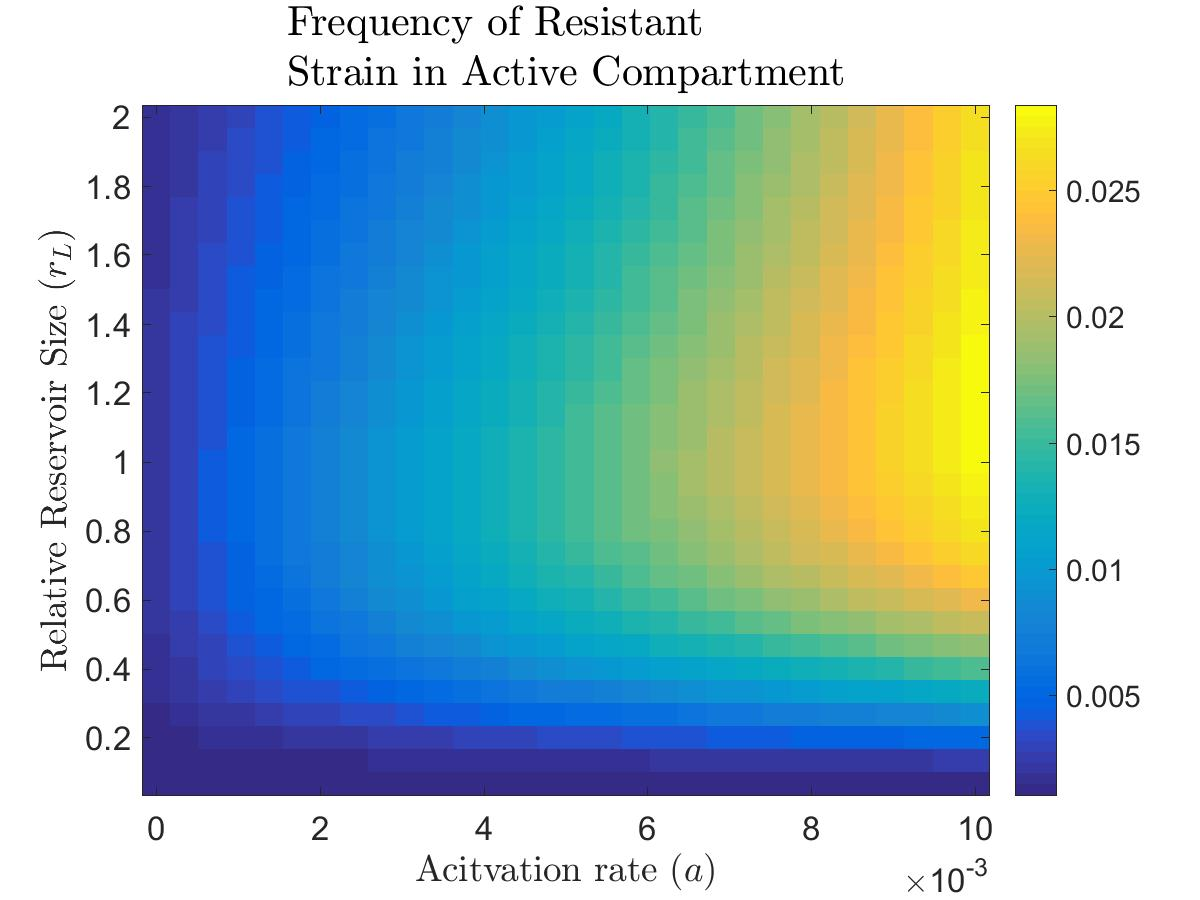
\includegraphics[width=0.75\textwidth]{FrequencyofResistantStraininActiveCompartment_19_04a.jpg}
\caption{Frequency of  the resistant strain present in the active compartment }
\label{fig:1} 
\end{figure*}


\begin{figure*}
\centering
  \includegraphics[width=.4\linewidth]
\centering  
  {FrequencyofResistantStraininActiveCompartment_19_04a.jpg}%
\centering
  \includegraphics[width=.4\linewidth]
\centering
  {FrequencyofResistantStraininActiveCompartment_19_04b.jpg}
\caption{Frequency of  the resistant strain present in the active compartment  in left pic it is with homestatic proliferation rate of zero. In the next we have $a = 0.01$. With the drug concebtration and reproduction rate as shown above}
\label{fig:1}
\end{figure*}



\begin{figure}
\begin{subfigure}{.5\textwidth}
  \centering
  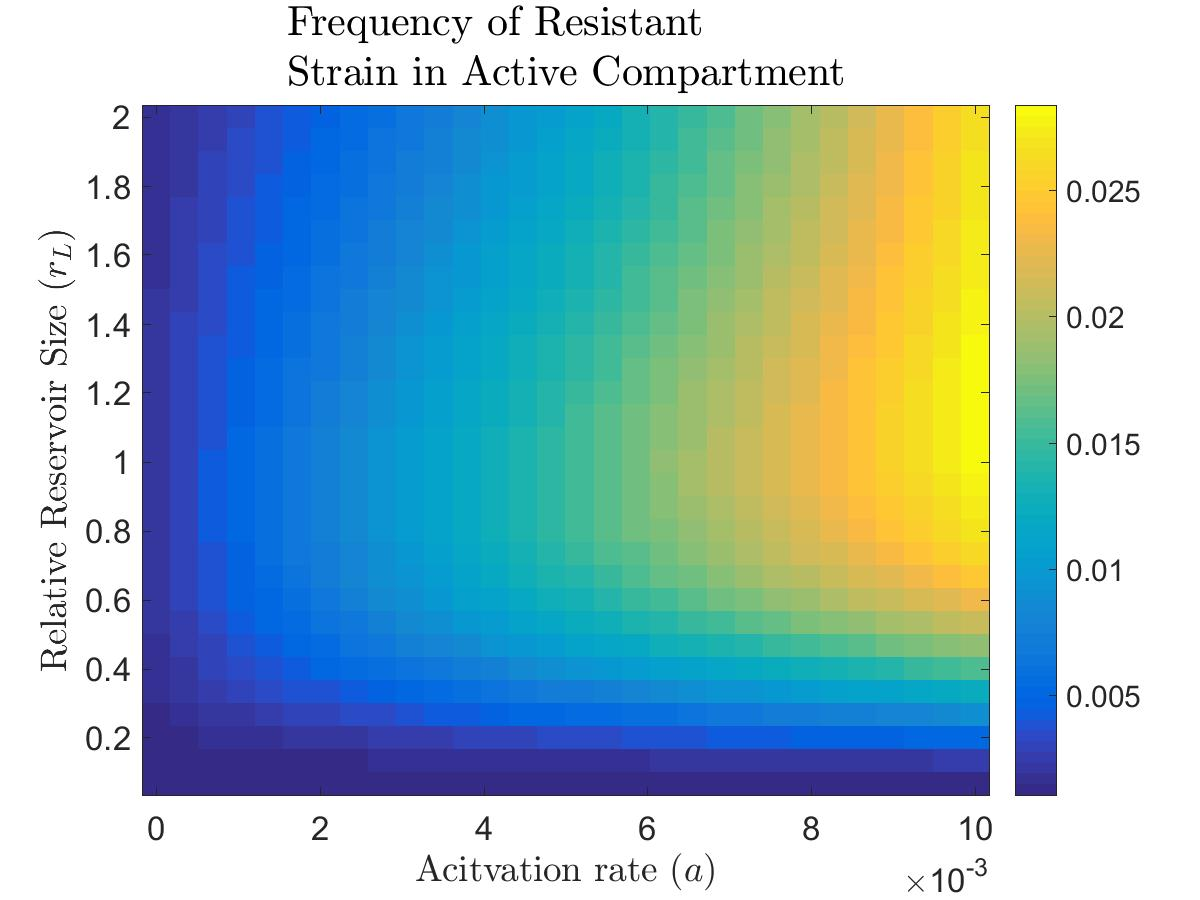
\includegraphics[width=.8\linewidth]{FrequencyofResistantStraininActiveCompartment_19_04a.jpg}
\end{subfigure}%
\begin{subfigure}{.5\textwidth}
  \centering
  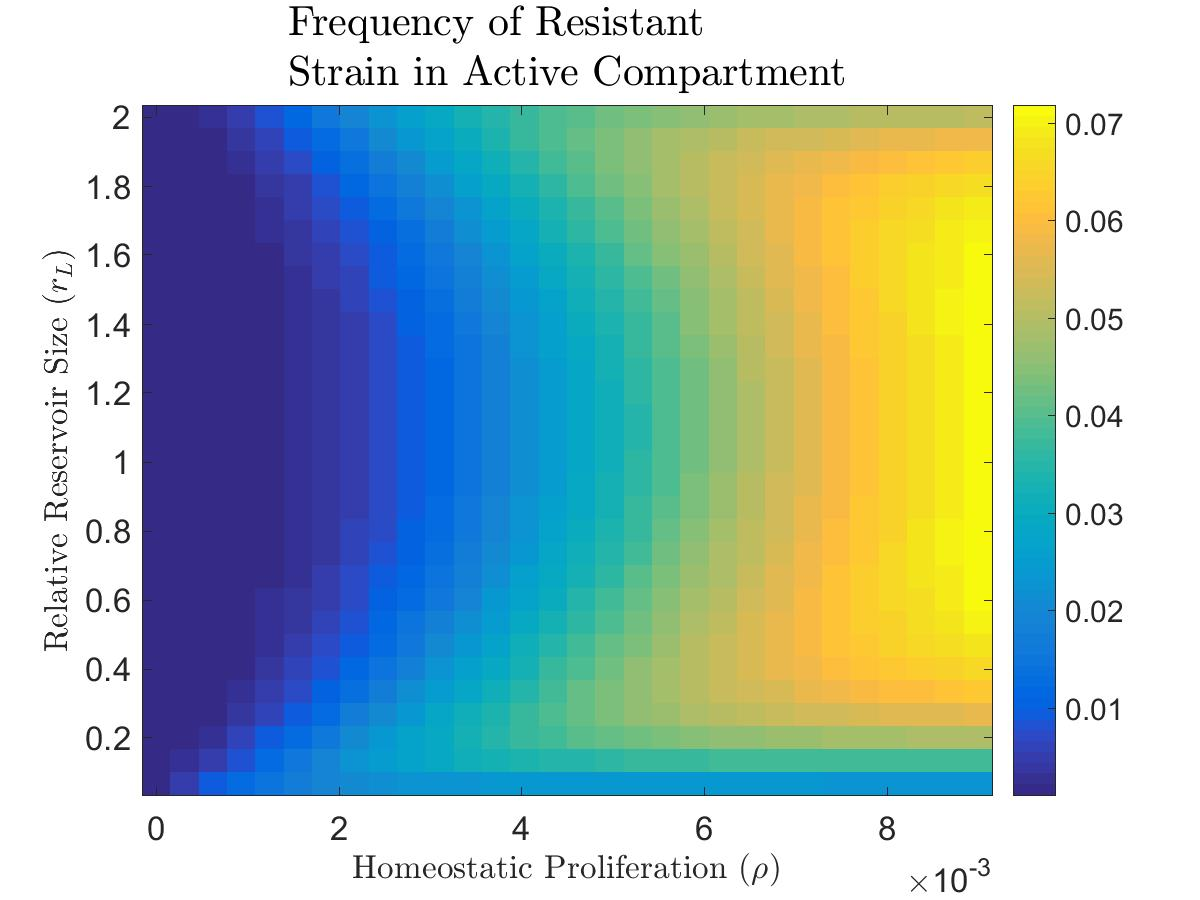
\includegraphics[width=.8\linewidth]{FrequencyofResistantStraininActiveCompartment_19_04b.jpg}
\end{subfigure}
\caption{plots of....}
\label{fig:fig}
\end{figure}

\fi


\iffalse
\begin{figure*}
% Use the relevant command to insert your figure file.
% For example, with the graphicx package use
  \includegraphics[width=0.75\textwidth]{WithinMultiHost.eps}
% figure caption is below the figure
\caption{within host dynamics for two host two strain system. Top  two are in host not on the drug, where blue is the wild type and red is  the resistant strain. In the bottom two the host is on PrEP,as we are dealing with frequencies initiating wth the wild type  in a host on pRep GIVES A FREQUENCY  of 1 for  the wild type  (but this is just relative) soitmay be good either to set the frequency to 0 if the actual amount is small enough (so it not add to 1) or the infectivity will need to take account of both the host transmitting the virus and the host getting it.}
\label{fig:noh}       % Give a unique label
\end{figure*}
\fi


\bibliographystyle{apa}
\bibliography{DTCProject1Bibliography}   % name your BibTeX data base



 
\end{document}